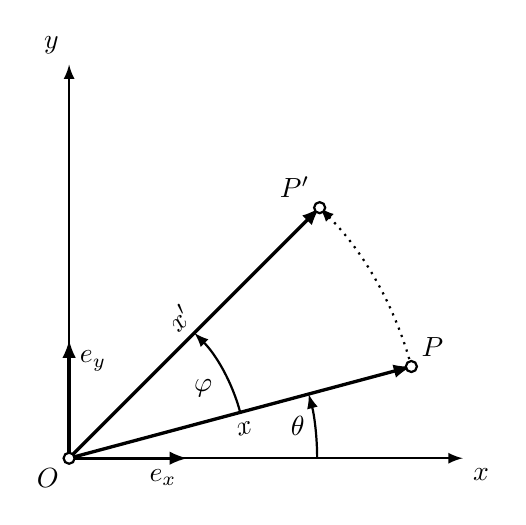
\begin{tikzpicture}
    %----------------------------------------------------------------------------------------%
    % Mathematik
    %----------------------------------------------------------------------------------------%
    \def\r{4.5};
    \def\u{30};
    \def\v{15};
    \pgfmathsetmacro\rxa{cos(\u)*\r};
    \pgfmathsetmacro\rya{sin(\u)*\r};
    \pgfmathsetmacro\rxb{cos(\v)*\rxa};
    \pgfmathsetmacro\ryb{sin(\v)*\rxa};
    %----------------------------------------------------------------------------------------%
    % Koordinaten
    %----------------------------------------------------------------------------------------%
    \coordinate (O) at (0,0);
    \coordinate (P1) at (\v:\r);
    \coordinate (P2) at (\v+\u:\r);
    %----------------------------------------------------------------------------------------%
    % Koordinatenachsen
    %----------------------------------------------------------------------------------------%
    \begin{scope}[thick,->,>=latex]
    \draw (O) -- +(5,0) node[anchor=north west] {$x$};
    \draw (O) -- +(0,5) node[anchor=south east] {$y$};
    \end{scope}
    %----------------------------------------------------------------------------------------%
    % Einheitsvektoren
    %----------------------------------------------------------------------------------------%
    \begin{scope}[very thick,->,>=latex,scale = 1.5]
    \draw (O) -- +(1,0) node[anchor = north east] {$\bvec{e_{x}}$};
    \draw (O) -- +(0,1) node[anchor = north west] {$\bvec{e_{y}}$};
    \end{scope}
    %----------------------------------------------------------------------------------------%
    % Vektoren
    %----------------------------------------------------------------------------------------%
    \begin{scope}[very thick,->,>=latex]
    \draw (O) -- (P1) node [midway, sloped, below] {$\bvec{x}$};
    \draw (O) -- (P2) node [midway, sloped, above] {$\bvec{x}^\prime$};
    \end{scope}
    %----------------------------------------------------------------------------------------%
    % Winkelbögen
    %----------------------------------------------------------------------------------------%
    \begin{scope}[thick,->,>=latex]
    \draw (P1)+(180+\v:\r/2) arc (\v:\v+\u:\r/2) node [midway, anchor = north east] {$\varphi$};
    \draw (0:\r*0.7) arc (0:\v:\r*0.7) node [midway, anchor = east] {$\theta$};
    \draw[dotted] (P1)+(180+\v:0) arc (\v:\v+\u:\r);
    \end{scope}
    %----------------------------------------------------------------------------------------%
    % Punkte
    %----------------------------------------------------------------------------------------%
    \begin{scope}[thick,draw=black,fill=white]
    \filldraw (O) circle (2pt) node[anchor=north east] {$O$};
    \filldraw (P1) circle (2pt) node[anchor=south west] {$P$};
    \filldraw (P2) circle (2pt) node[anchor=south east] {$P^\prime$};
    \end{scope}
    %----------------------------------------------------------------------------------------%
\end{tikzpicture}